\section{Мета роботи}
Набути практичного досвіду та закріпити знання про подання
стека, дека, пріоритетної черги та дисципліни їх обслуговування.

\section{Хід роботи}
  Розробити функції, що забезпечують запис та читання запитів із
пріоритетної черги, стека або дека.

  В кожному завданні для організації вказаної черги використати дві
структури. Перевірити працездатність розроблених функцій. Послідовність
виконання операцій запису та читання обирати випадково.\\

\textbf{Моє завдання:}
  Пріоритетна черга. Постановка запитів у чергу виконується за
пріоритетом, зняття – підряд зі старших адрес (кінця черги). Черга
організована на масиві та на списку. Пріоритет: mах значення числового
параметра; при збігу параметрів – FIFO.

\clearpage
\subsection{Реалізація черги на базі масиву}
	Було реалізовано такі методи: \textit{ініціалізація черги, додавання у кінець черги, 
вивід черги, видалення з початку черги, знищення черги.}

\begin{lstlisting}[style=customc]
#include <stdio.h>
#include <stdlib.h>

typedef struct
{
  int data;
  int priority;
} PriorityQueueElement;

// Array based priority queue
typedef struct
{
  PriorityQueueElement *elements;
  int size;
  int capacity;
  int front;
  int rear;
  size_t allocated_memory;
} PriorityQueue;

PriorityQueue init_priority_queue(int capacity)
{
  PriorityQueue pq;
  pq.elements =
      (PriorityQueueElement *)malloc(sizeof(PriorityQueueElement) * capacity);
  pq.size = 0;
  pq.capacity = capacity;
  pq.front = 0;
  pq.rear = 0;
  pq.allocated_memory = sizeof(PriorityQueueElement) * capacity;
  return pq;
}

void resize(PriorityQueue *pq)
{
  pq->capacity *= 2;
  pq->elements = (PriorityQueueElement *)realloc(
      pq->elements, sizeof(PriorityQueueElement) * pq->capacity);
  pq->allocated_memory = sizeof(PriorityQueueElement) * pq->capacity;
}

void push_priority_queue(PriorityQueue *pq, int data, int priority)
{
  if (pq->size == pq->capacity)
  {
    resize(pq);
  }

  PriorityQueueElement newElem = {data, priority};

  int i = pq->size - 1;

  while (i >= 0 && pq->elements[i].priority < priority)
  {
    pq->elements[i + 1] = pq->elements[i];
    i--;
  }

  pq->elements[i + 1] = newElem;
  pq->size++;
}

PriorityQueueElement pop_priority_queue(PriorityQueue *pq)
{
  if (pq->size == 0)
  {
    printf("Priority queue is empty.\n");
    PriorityQueueElement emptyElement = {0, 0};
    return emptyElement;
  }

  PriorityQueueElement topElement = pq->elements[pq->front];

  for (int i = 0; i < pq->size - 1; i++)
  {
    pq->elements[i] = pq->elements[i + 1];
  }

  pq->size--;
  return topElement;
}

void destroy_priority_queue(PriorityQueue *pq)
{
  free(pq->elements);
  pq->allocated_memory = 0;
}

void print_priority_queue(PriorityQueue *pq)
{
  if (pq->size == 0)
  {
    printf("Priority queue is empty.\n");
    return;
  }

  for (int i = 0; i < pq->size; i++)
  {
    printf("Value: %d, Priority: %d", pq->elements[i].data, pq->elements[i].priority);
    if (i < pq->size - 1)
    {
      printf("\n");
    }
  }
  printf("\n");
}
\end{lstlisting}

\clearpage
\subsection{Реалізація черги на базі списку}
Дана структура була побудована на базі перевикористовуваного зв`язного списку який буде наведено нижче.\\

  Було реалізовано такі методи: \textit{ініціалізація черги, додавання у кінець черги, 
вивід черги, видалення з початку черги, знищення черги.}
  
\begin{lstlisting}[style=customc]
#include "priority_queue_list.h"
#include <stdlib.h>
#include <stdio.h>

static int compare_priority(const void *a, const void *b)
{
  const LPQElement *elemA = (const LPQ *)a;
  const LPQElement *elemB = (const LPQ *)b;

  if (elemA->priority != elemB->priority)
  {
    return elemB->priority - elemA->priority; // Max priority first
  }
  return 0; // FIFO when priority same
}

static void free_lpq_element(void *data)
{
  free(data);
}

static void print_lpq_element(const void *data)
{
  const LPQElement *elem = (const LPQ *)data;
  printf("Value: %d, Priority: %d\n", elem->value, elem->priority);
}

LPQ *init_lpq()
{
  LPQ *queue = (LPQ *)malloc(sizeof(LPQ));
  if (!queue)
  {
    perror("Cannot able to allocate memory!");
    exit(EXIT_FAILURE);
  }
  queue->head = NULL;
  queue->allocated_memory = sizeof(LPQ);
  return queue;
}

void enqueue_lpq(LPQ *queue, int value, int priority)
{
  LPQElement *newElement = (LPQElement *)malloc(sizeof(LPQElement));
  if (!newElement)
  {
    perror("Cannot able to allocate memory!");
    exit(EXIT_FAILURE);
  }
  newElement->value = value;
  newElement->priority = priority;

  queue->allocated_memory += sizeof(LPQElement);

  Node **head = &(queue->head);

  if (!*head || compare_priority((*head)->data, newElement) > 0)
  {
    insert_head_linked_list(head, newElement);
  }
  else
  {
    Node *current = *head;
    while (current->next && compare_priority(current->next->data, newElement) <= 0)
    {
      current = current->next;
    }
    insert_after_element_linked_list(current, newElement);
  }
}

int dequeue_lpq(LPQ *queue)
{
  if (!queue->head)
  {
    printf("Queue is empty!\n");
    return -1;
  }
  LPQElement *top = (LPQElement *)queue->head->data;
  int value = top->value;
  queue->allocated_memory -= sizeof(LPQElement);

  delete_node_linked_list(&(queue->head), top, compare_priority, free_lpq_element);
  return value;
}

void destroy_lpq(LPQ *queue)
{
  destroy_linked_list(&(queue->head), free_lpq_element);
  free(queue);
  queue->allocated_memory = 0;
}

void print_lpq(LPQ *queue)
{
  print_linked_list(queue->head, print_lpq_element);
}
\end{lstlisting}


\clearpage
\subsection{Реалізація універсального зв`язного списку}
  Він є універсальним бо не має визначений тип даних для зберігання,
а зберігає пустий вказівник, що дає змогу хранити там будь-що. \\

Також можна перевизначити певні методи що дає також універсальність використання.

\begin{lstlisting}[style=customc]
#include "linked_list.h"
#include <stdio.h>
#include <stdlib.h>

Node *create_node_linked_list(void *data)
{
  Node *newNode = (Node *)malloc(sizeof(Node));
  if (!newNode)
  {
    perror("Cannot able to allocate memory!\n");
    exit(EXIT_FAILURE);
  }
  newNode->data = data;
  newNode->next = NULL;
  return newNode;
}

void insert_head_linked_list(Node **head, void *data)
{
  Node *newNode = create_node_linked_list(data);
  newNode->next = *head;
  *head = newNode;
}

void insert_after_element_linked_list(Node *node, void *data)
{
  if (!node)
    return;
  Node *newNode = create_node_linked_list(data);
  newNode->next = node->next;
  node->next = newNode;
}

void delete_node_linked_list(Node **head, void *target, CompareFunc comparer, void (*free_data)(void *))
{
  if (!head || !*head)
    return;

  Node *temp = *head;
  Node *prev = NULL;

  while (temp && comparer(temp->data, target) != 0)
  {
    prev = temp;
    temp = temp->next;
  }

  if (!temp)
    return;

  if (prev)
  {
    prev->next = temp->next;
  }
  else
  {
    *head = temp->next;
  }

  if (free_data)
  {
    free_data(temp->data);
  }
  free(temp);
}

Node *find_element_linked_list(Node *head, void *target, CompareFunc comparer)
{
  while (head)
  {
    if (comparer(head->data, target) == 0)
    {
      return head;
    }
    head = head->next;
  }
  return NULL;
}

void destroy_linked_list(Node **head, void (*free_data)(void *))
{
  while (*head)
  {
    Node *temp = *head;
    *head = (*head)->next;

    if (free_data)
    {
      free_data(temp->data);
    }
    free(temp);
  }
}

void print_linked_list(Node *head, void (*print_data)(const void *))
{
  while (head)
  {
    print_data(head->data);
    head = head->next;
  }
}
\end{lstlisting}

\clearpage
\subsection{Реалізація лабораторної програми}
Було протестовано дві структури даних та порівняно за кількість використаної пам`яті.

\begin{lstlisting}[style=customc]
#include <stdio.h>
#include <stdlib.h>

#include "general_utils.h"
#include "priority_queue_arr.h"
#include "priority_queue_list.h"

void task1()
{
  PriorityQueue pq = init_priority_queue(5);
  LPQ *lpq = init_lpq();

  push_priority_queue(&pq, 10, 1);
  push_priority_queue(&pq, 20, 4);
  push_priority_queue(&pq, 15, 2);
  push_priority_queue(&pq, 69, 5);

  enqueue_lpq(lpq, 10, 1);
  enqueue_lpq(lpq, 20, 4);
  enqueue_lpq(lpq, 15, 2);
  enqueue_lpq(lpq, 69, 5);

  highlightText("Elements of LIST base priority queue:\n", "blue");
  print_lpq(lpq);
  printf("Memory allocated: \033[34m%zu\033[0m bytes\n", lpq->allocated_memory);
  puts("");

  highlightText("Elements of ARRAY priority queue:\n", "blue");
  print_priority_queue(&pq);
  printf("Memory allocated: \033[32m%zu\033[0m bytes\n", pq.allocated_memory);
  puts("");

  highlightText("Adding new element with highest priority to LIST priority queue:\n", "yellow");
  enqueue_lpq(lpq, 100, 10);
  print_lpq(lpq);
  printf("Memory allocated: \033[32m%zu\033[0m bytes\n", lpq->allocated_memory);
  puts("");

  highlightText("Adding new element with highest priority to ARRAY priority queue:\n", "yellow");
  push_priority_queue(&pq, 100, 10);
  print_priority_queue(&pq);
  printf("Memory allocated: \033[32m%zu\033[0m bytes\n", pq.allocated_memory);
  puts("");

  highlightText("Adding new element with similar priority to LIST priority queue:\n", "blue");
  enqueue_lpq(lpq, 777, 2);
  print_lpq(lpq);
  printf("Memory allocated: \033[32m%zu\033[0m bytes\n", lpq->allocated_memory);
  puts("");

  highlightText("Adding new element with similar priority to ARRAY priority queue:\n", "blue");
  push_priority_queue(&pq, 777, 2);
  print_priority_queue(&pq);
  printf("Memory allocated: \033[32m%zu\033[0m bytes\n", pq.allocated_memory);
  puts("");

  highlightText("Pop 4 elements from LIST priority queue:\n", "yellow");
  dequeue_lpq(lpq);
  dequeue_lpq(lpq);
  dequeue_lpq(lpq);
  dequeue_lpq(lpq);
  print_lpq(lpq);
  printf("Memory allocated: \033[32m%zu\033[0m bytes\n", lpq->allocated_memory);
  puts("");

  highlightText("Pop 4 elements from ARRAY priority queue:\n", "yellow");
  pop_priority_queue(&pq);
  pop_priority_queue(&pq);
  pop_priority_queue(&pq);
  pop_priority_queue(&pq);
  print_priority_queue(&pq);
  printf("Memory allocated: \033[32m%zu\033[0m bytes\n", pq.allocated_memory);
  puts("");

  destroy_lpq(lpq);
  destroy_priority_queue(&pq);
}
\end{lstlisting}


\clearpage
\subsection{Результати роботи програми:}

\begin{figure}[h!]
    \centering
    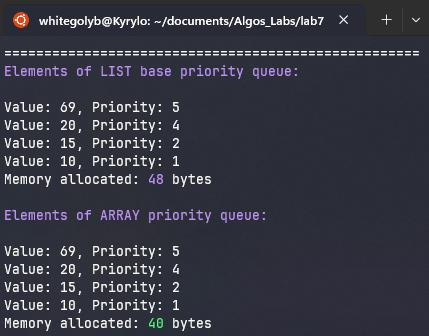
\includegraphics[width=15cm]{reports/algos/lab7/assets/1.jpeg}
    \caption{Занесення елементів у черги}
\end{figure}


\begin{figure}[h!]
  \centering
  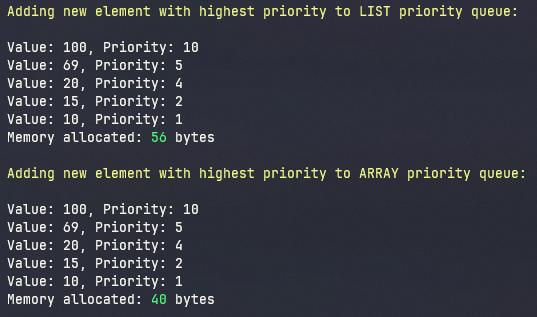
\includegraphics[width=15cm]{reports/algos/lab7/assets/2.jpeg}
  \caption{Додавання нового елемента з найвищим пріорітетом}
\end{figure}

\begin{figure}[h!]
  \centering
  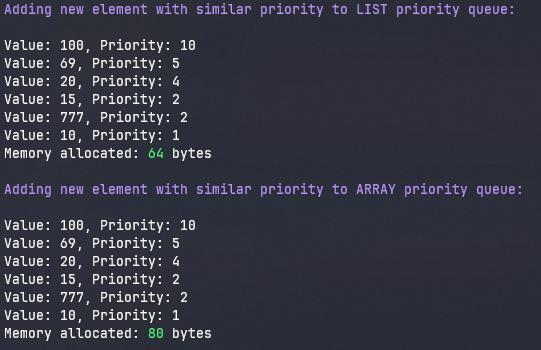
\includegraphics[width=15cm]{reports/algos/lab7/assets/3.jpeg}
  \caption{Додавання елемента вже з існуючим пріорітетом}
\end{figure}

\begin{figure}[h!]
  \centering
  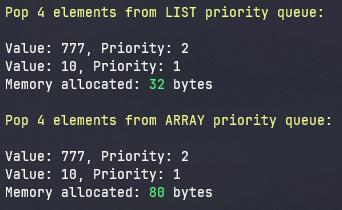
\includegraphics[width=15cm]{reports/algos/lab7/assets/4.jpeg}
  \caption{Видалення 4 елементів з черг}
\end{figure}

\clearpage
\section{Висновки}
  В ході виконання лабораторної роботи було розроблено дві структури даних відповідно свого
варіанту.\\

  Можна зазначити що всі структури даних працюють коректно та мають однаковий інтерфейс,
але різну реалізацію.\\

Черга на базі масиву виділяє неперервну ділянку пам`яті заздалегідь під декілька елементів, що може 
бути корисно коли черга заздалегідь визначена, швидкість доступу за індексом до елементів буде швидше.\\

  Черга на базі списку виділя пам`ять для кожного елементу окремо але не неперервно, це добре коли 
черга невизначена на може динамічно змінюватися, також швидше буде працювати операція видалення та додавання елементів.\\

Порівняння використаної пам`яті можна побачити на скріншотах результатів.



